\chapter{Mechanical Design}
The robot meets the Roborodentia design requirements shown in Table \ref{tab:roborodentia_reqs}. It consists of four subassemblies: the base platform, shooting mechanism, ball hopper, and control unit. Each section was modeled in SolidWorks, an industry-standard solid modeling CAD program \cite{3dhubs}\cite{solidworks}. The parts were then fabricated using a laser cutter or 3D printer and assembled with metric hardware. Figure \ref{fig:robot_photo} displays a photograph of the robot while Figures \ref{fig:render_isometric} through \ref{fig:render_right} show standard view renders of the SolidWorks model. Note that the robot uses mecanum wheels (a type of omni-directional wheel) which are modeled as plain wheels for simplicity \cite{ilon_1975}. Figure \ref{fig:render_top} also indicates the front, left, back/rear, and right sides of the robot as referenced in the rest of the paper.  The robot contains 53 different mechanical components (including fasteners and off-the-shelf parts), of which 24 are custom designed, and 394 parts in total. The bill of materials can be found in Appendix \ref{appendix:mech_bom}.

\begin{table}[h]
	\caption{Roborodentia 2018 Mechanical Requirements}  \label{tab:roborodentia_reqs}
	\begin{tabularx}{\textwidth}{@{} c Y @{}}
		\toprule
		& Requirement \\ 
		\midrule
		1. & Maximum footprint of 12" x 14" or smaller at start of match but may expand up to 14" x 17" during match. \\
		2. & Maximum height of 14" at start of match but no restriction during match. \\ 
		3. & Robot may not disassemble into multiple parts. \\ 
		4. & Robot may not be airborne. \\ 
		5. & Shooting mechanisms may not accelerate balls past 50 feet per second. \\ 
		\bottomrule
	\end{tabularx} 
\end{table}

\begin{figure}[H]   % [h] means here
	\centering \includegraphics[width=6in, height=7in, keepaspectratio]{figures/robot_photo.png}
	\caption{Photograph of Robot}	\label{fig:robot_photo}
\end{figure}
\begin{figure}[H]   % [h] means here
	\centering 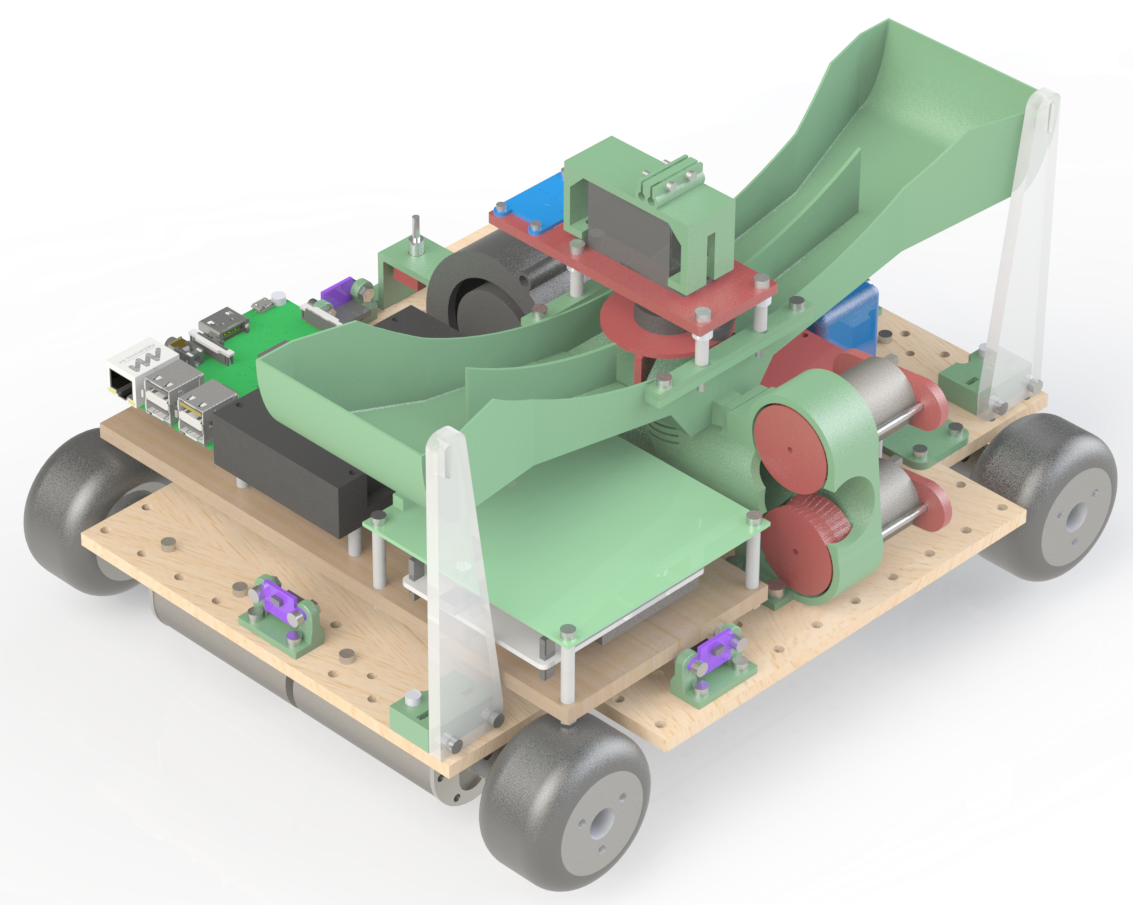
\includegraphics[width=6in, height=3.85in, keepaspectratio]{figures/render_isometric.png}
	\caption{Full Robot Render -- Isometric View}\label{fig:render_isometric}
\end{figure}
\begin{figure}[H]   % [h] means here
	\centering 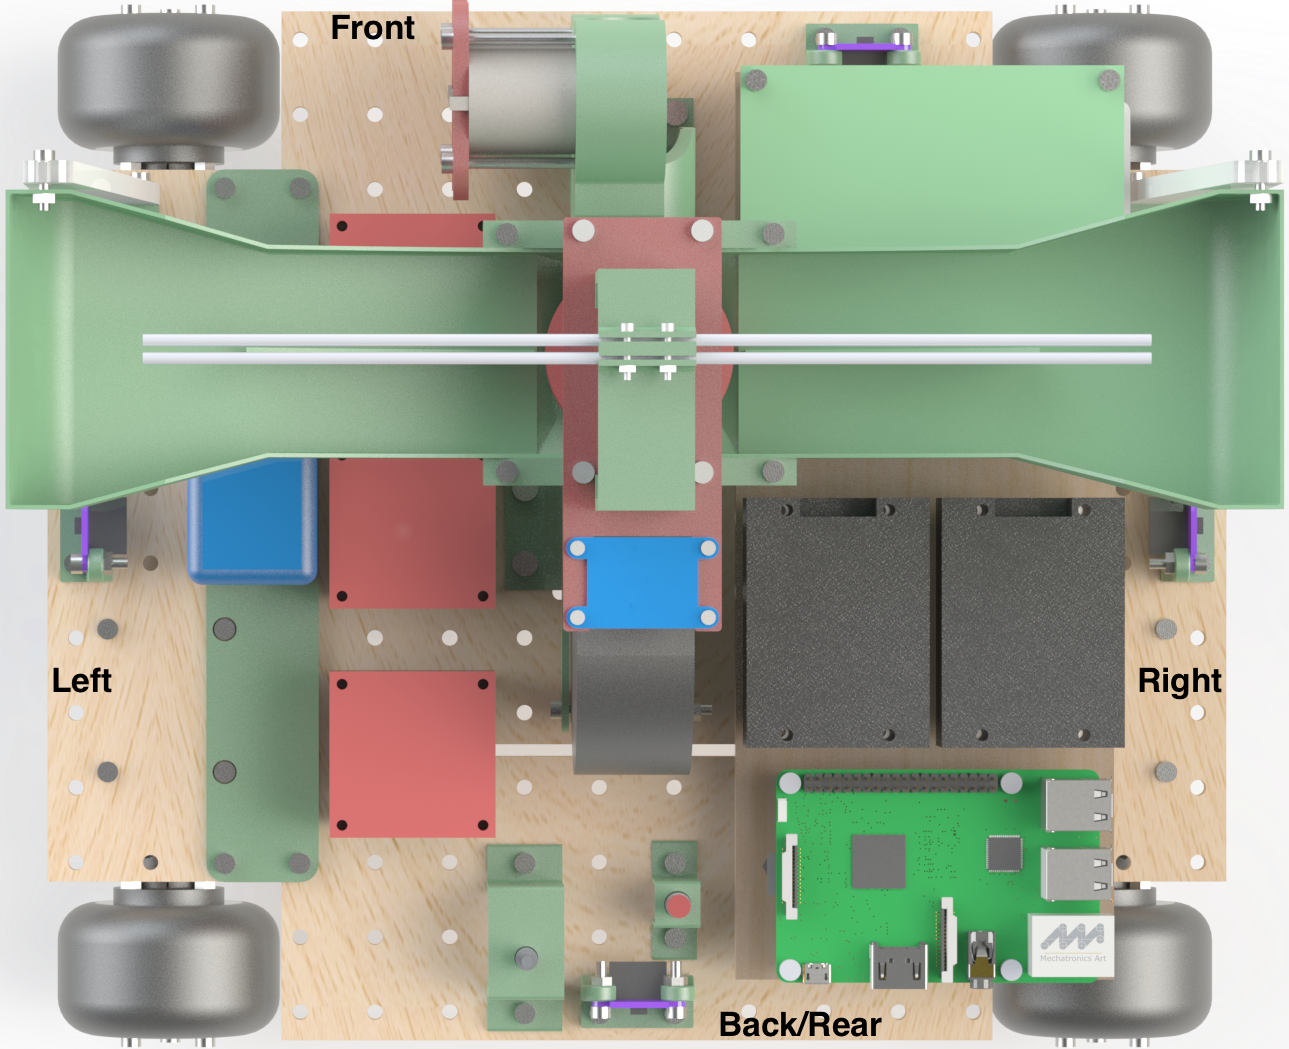
\includegraphics[width=6in, height=3.85in, keepaspectratio]{figures/render_top.png}
	\caption{Full Robot Render -- Top View}	\label{fig:render_top}
\end{figure}
\begin{figure}[H]   % [h] means here
	\centering 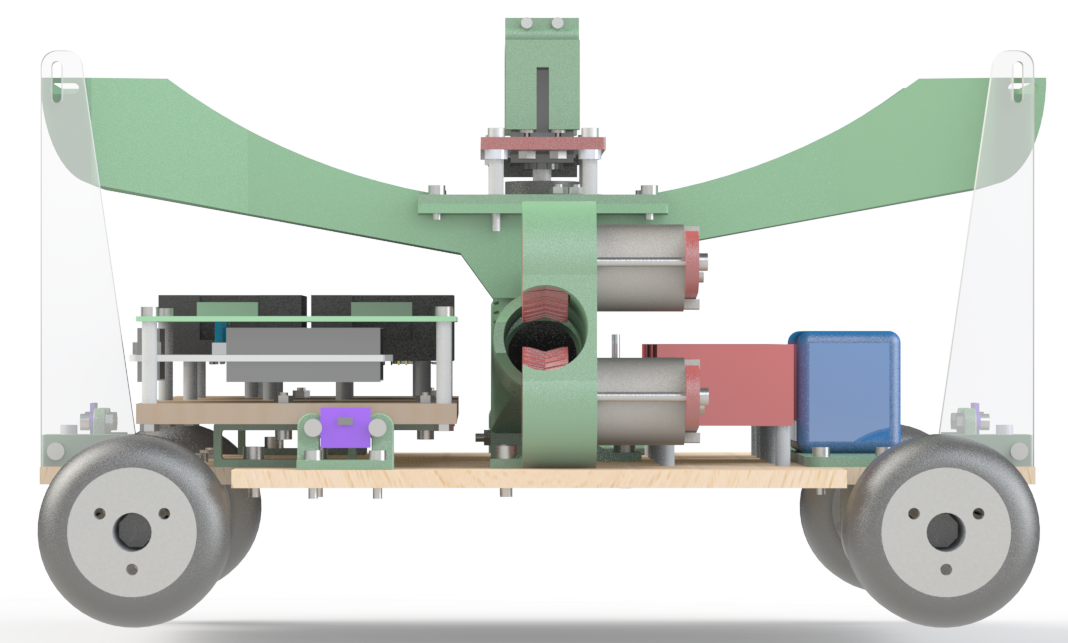
\includegraphics[width=6in, height=3.85in, keepaspectratio]{figures/render_front.png}
	\caption{Full Robot Render -- Front View}	\label{fig:render_front}
\end{figure}
\begin{figure}[H]   % [h] means here
	\centering 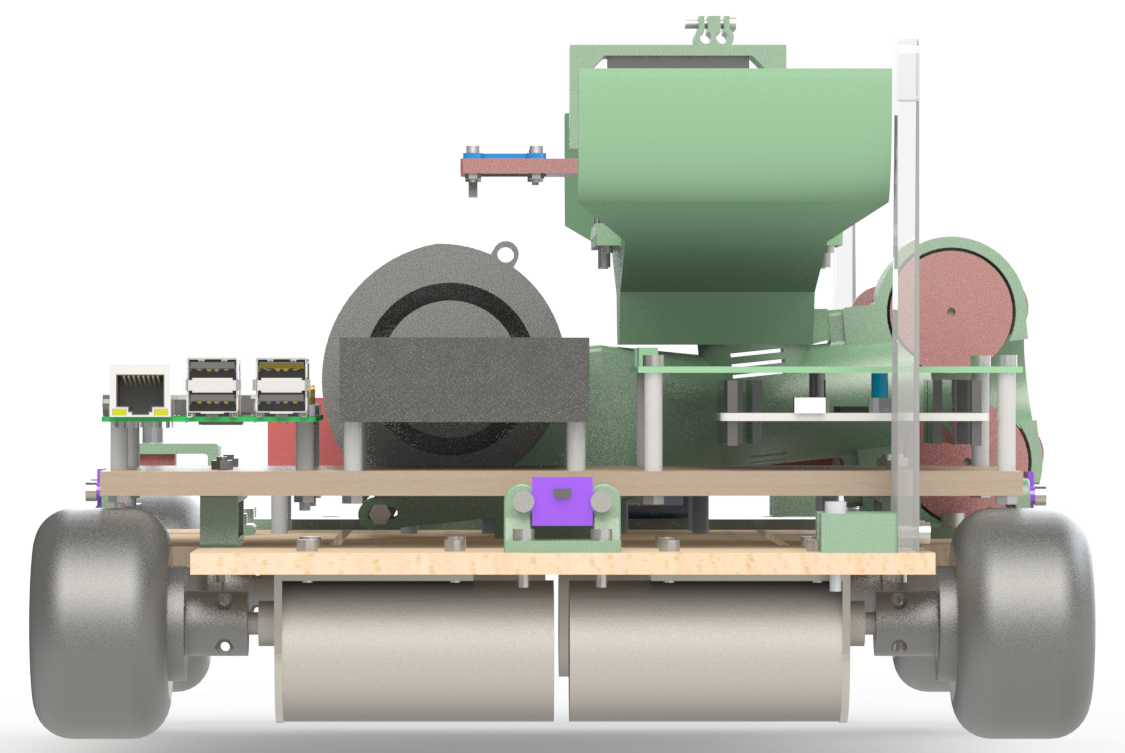
\includegraphics[width=6in, height=3.85in, keepaspectratio]{figures/render_right.png}
	\caption{Full Robot Render -- Right View}	\label{fig:render_right}
\end{figure}

The design emphasizes the use of 3D-printed parts to take advantage of the benefits of the technology including rapid part production, high part complexity, and low fabrication cost (excluding the cost of the printer, relative to other methods such as machining, casting, and injection molding), ideal for one-off part production. Parts were printed on a MakerGear M2 fused deposition modeling (FDM) 3D printer equipped with a 0.35 mm diameter nozzle using MakerGeeks 1.75 mm ABS thermoplastic filament \cite{makergear_m2}\cite{makergeeks}. Print speeds of 20 to 80 mm/s with 0.20 mm layer height, depending on part dimensions and minimum feature size, lead to part print times of 2--5 hours for smaller components and up to 26 hours for the ball hopper. Due to the non-isotropic strength characteristic of 3D-printed components, the designs must specifically take into account printing direction and orientation. Parts tend to possess greater tensile strength in the X and Y axes but significantly less in the Z direction \cite{3dhubs_orientation}. Additionally, the print volume of 200 mm x 250 mm x 200 mm limits the maximum part dimensions, requiring the ball hopper to printed as three separate pieces \cite{makergear_m2}. 

\section{Base Platform}
The 315 mm x 275 mm base platform of the robot, made from 1/4" thick medium density fiberboard (MDF), serves as the primary structural component and mounting point for the motors, electronics, shooting mechanism, and hopper. The wood is laser cut with a 20 mm grid of 4 mm diameter holes to allow modular placement of components. The corner cutouts allow clearance for the wheels. Long slots permit wire routing from the motors to the motor drivers above. Figure \ref{fig:base_platform} shows the subassembly with labels.

\begin{figure}[H]   % [h] means here
	\centering 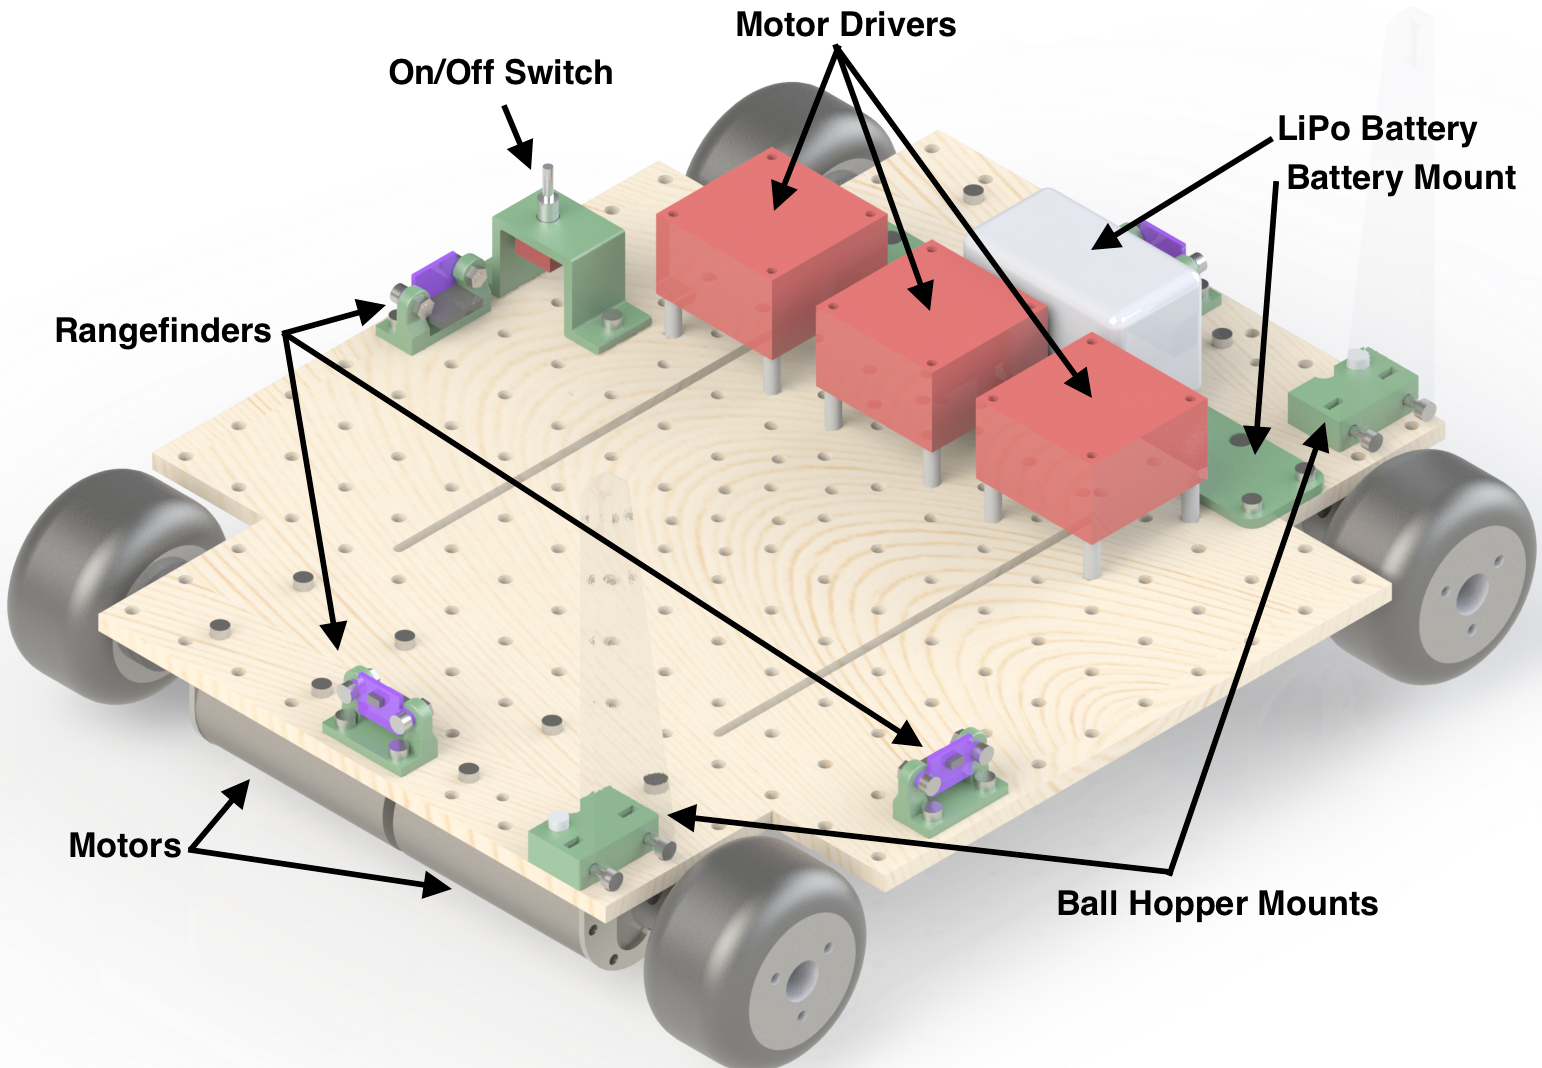
\includegraphics[width=6in, height=3.85in, keepaspectratio]{figures/base_platform.png}
	\caption{Base Platform}	\label{fig:base_platform}
\end{figure}

Four 12V Pololu 37D motors geared at a 70:1 ratio drive each of the 60 mm diameter mecanum wheels \cite{pololu}. Figure \ref{fig:motor_assem_explode} displays an exploded view of the motor assembly. 3D-printed couplings, detailed in Figure \ref{fig:wheel_coupler}, connect the wheels to the 6 mm diameter, D-shaped motor shafts. The couplers use M2 nuts and bolts to clamp onto the motor shaft and an octagonal stub that press fits into the center of the wheels. Three long M3 bolts and nylon lock nuts clamp the mecanum wheels together and to the coupler. Each wheel contains eight angled rollers mounted with two ball bearings each to smooth operation under load. Unlike regular wheels which only produce a force vector perpendicular to the axis, mecanum wheels also produce a vector parallel to the axis. With the appropriate combination of speed and direction of each wheel, the robot can achieve simultaneous translation and rotation in any direction. 

\begin{figure}[H]   % [h] means here
	\centering 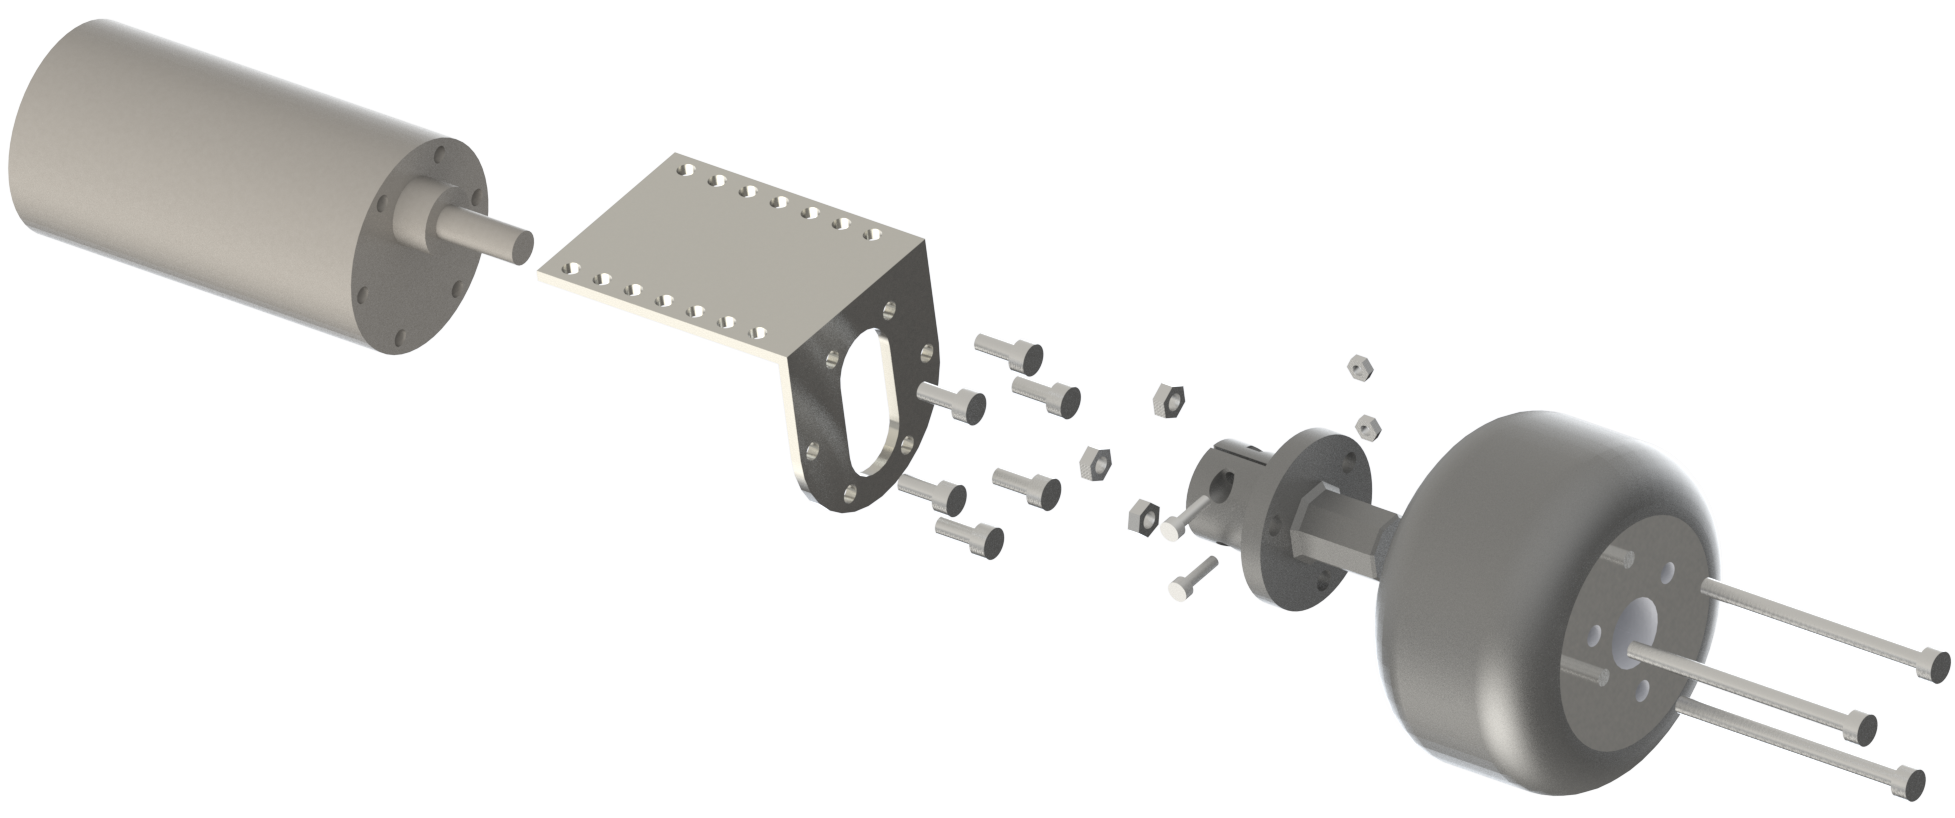
\includegraphics[width=6in, height=3.85in, keepaspectratio]{figures/motor_assem_explode.png}
	\caption{Motor Assembly Exploded View}	\label{fig:motor_assem_explode}
\end{figure}
\begin{figure}[H]   % [h] means here
	\centering 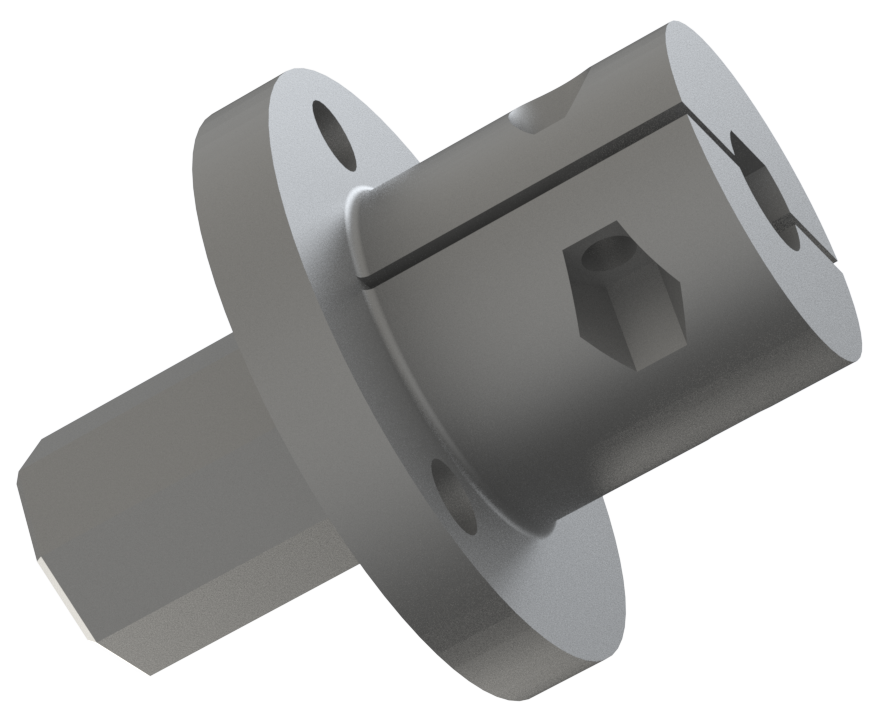
\includegraphics[width=3in, height=3.85in, keepaspectratio]{figures/wheel_coupler.png}
	\caption{Wheel Coupler}	\label{fig:wheel_coupler}
\end{figure}

Four STMicroelectronics VL53L0X laser rangefinders on the robot periphery sense distances between 30 mm and 2000 mm at a rate of 30 Hz and provide less than 10\% error in most test conditions \cite{vl53l0x_datasheet}. A 4S, 1800 mAH LiPo battery mounted with an industrial strength hook-and-loop fastener powers the system through a on/off toggle switch seated in a 3D-printed bracket \cite{battery}. Three dual H-bridge motor drivers are attached with nylon standoffs and M3 nuts and bolts. Finally, a momentary push button in a 3D-printed bracket toggles power to the Raspberry Pi microcomputer.

\section{Shooting Mechanism}
The competition calls for robots to fire Nerf Rival Balls into large nets positioned several feet away. The shooting mechanism takes inspiration from the official Nerf Rival Blaster toys since they're specifically optimized to fire Nerf Rival balls; the system works similarly to a baseball pitching machine. Figure \ref{fig:shooter_explode} shows an exploded view of the robot's shooter subassembly while Figure \ref{fig:shooter_top} displays the top view. The mechanism consists of two sections: the \textbf{barrel} and the \textbf{wheel housing}. Both parts were 3D-printed as the geometries are highly complex. Therefore, the shooting mechanism consists of two separate components versus a unibody design to allow each half to be fabricated with optimal print direction, strength, and finish quality. The barrel is angled \ang{6} above horizontal, targeting the vertical center of the nets 6 feet away.

\begin{figure}[H]   % [h] means here
	\centering 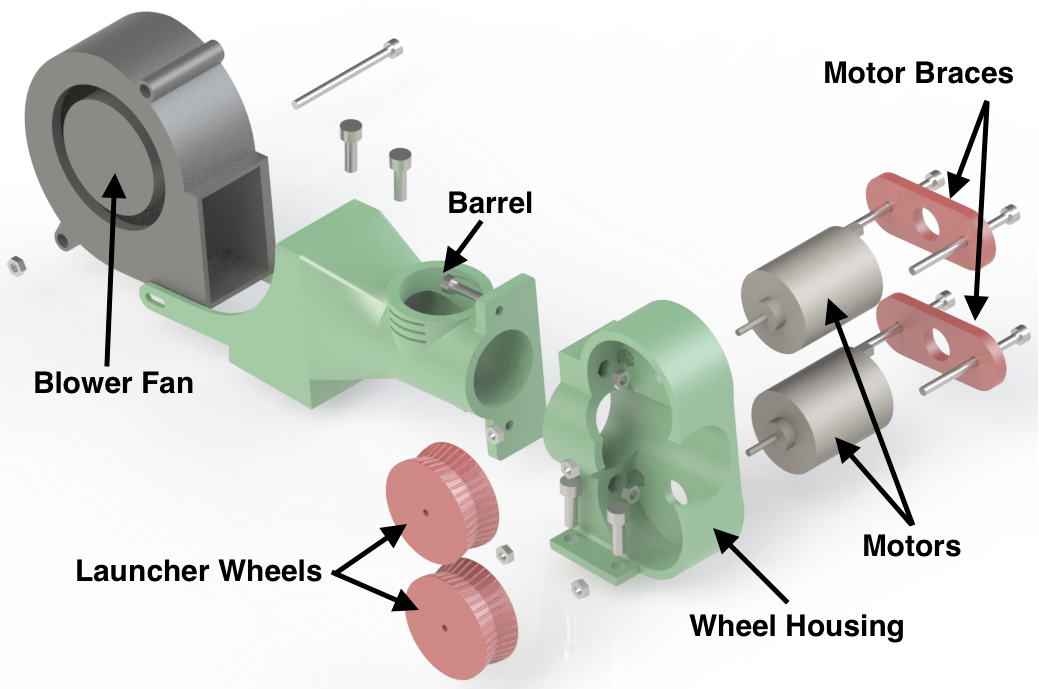
\includegraphics[width=6in, height=3.85in, keepaspectratio]{figures/shooter_explode.png}
	\caption{Shooting Mechanism -- Exploded View}	\label{fig:shooter_explode}
\end{figure}
\begin{figure}[H]   % [h] means here
	\centering 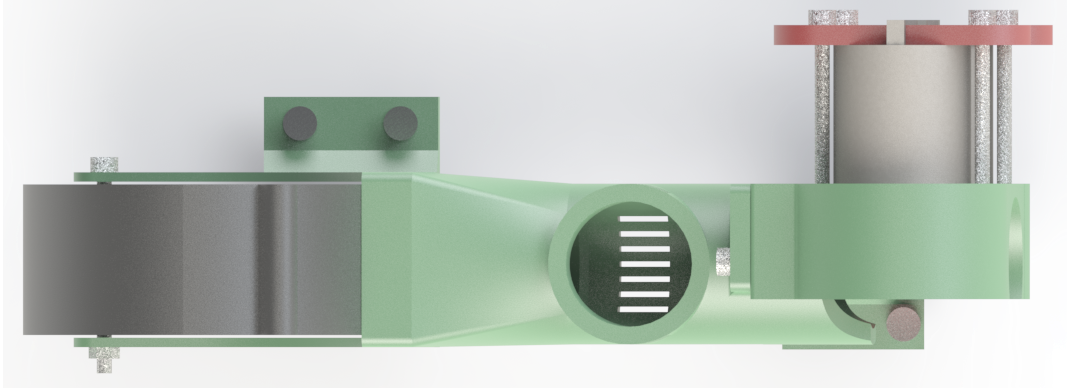
\includegraphics[width=6in, height=3.85in, keepaspectratio]{figures/shooter_top.png}
	\caption{Shooting Mechanism -- Top View}	\label{fig:shooter_top}
\end{figure}

The \textbf{barrel} directs balls from the \textbf{ball hopper} to the \textbf{wheel housing}. First, the ball enters the barrel through a vertical chute by force of gravity. As the ball falls into the barrel, a high-pressure centrifugal (or blower fan) attached at the back of the barrel pushes it into the wheel housing inlet. As seen in Figure \ref{fig:shooter_xsec}, the barrel slightly narrows in the area behind the top chute to prevent the ball from rolling backwards towards the blower fan. A 3D-modeling feature called a boss/base loft creates a smooth transition between the rectangular fan inlet and the circular barrel \cite{zuyderduyn_2016}. The foam balls, nominally 23 mm in diameter, would occasionally jam in a 24 mm inner diameter barrel due to ball surface imperfections, so the barrel was increased to 25 mm inner diameter. In the initial design, the pressure created by the blower fan was so high that it prevented the ball from falling down the vertical chute. The revised barrel uses strategically placed vents to reduce pressure before the ball enters the chute. As the ball travels down the chute into the barrel, it blocks the vents, increasing the pressure and forcing itself into the wheel housing.

\begin{figure}[H]   % [h] means here
	\centering 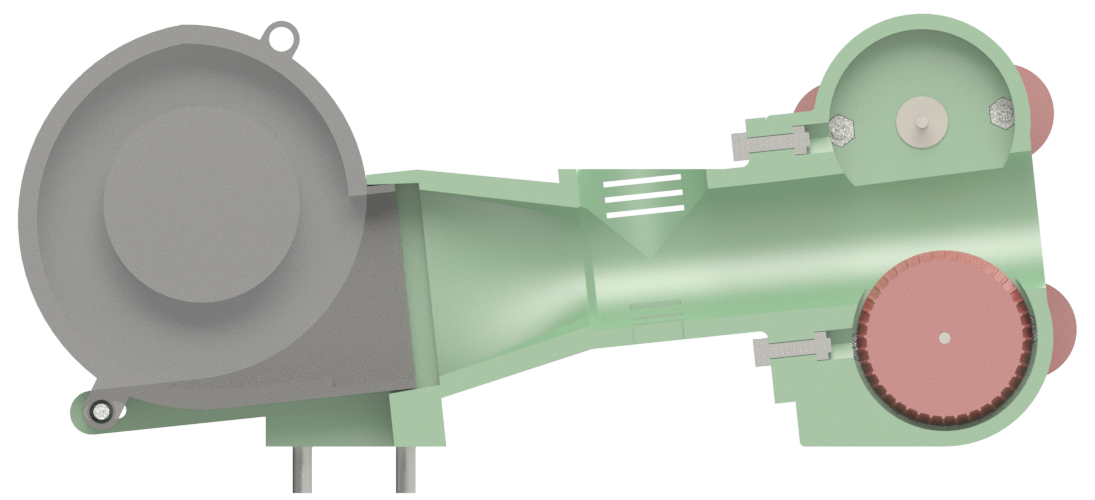
\includegraphics[width=6in, height=3.85in, keepaspectratio]{figures/shooter_xsec.png}
	\caption{Shooting Mechanism -- Cross Section View}	\label{fig:shooter_xsec}
\end{figure}

Inside the \textbf{wheel housing}, two counter-rotating 34mm wheels press fitted to two high-speed 12 V motors rapidly accelerate the foam ball up to 50 feet per second. The 14 mm gap between wheels compresses the ball to increase grip, thereby improving energy transfer. The motors lightly press fit into the wheel housing and are secured with 3D-printed braces. The perimeter of each 3D-printed wheel, detailed in Figure \ref{fig:shooter_wheel}, consists of a ribbed V-groove to increase the contact patch and grip with the compressed foam ball. Two "feet" with bolt holes at the bottom of the barrel and wheel housing secure the shooting mechanism to the base platform.

\begin{figure}[H]   % [h] means here
	\centering 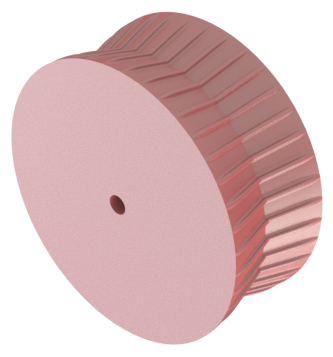
\includegraphics[width=6in, height=3.85in, keepaspectratio]{figures/shooter_wheel.png}
	\caption{Shooting Mechanism -- Shooter Wheel}	\label{fig:shooter_wheel}
\end{figure}

The shooting mechanism performed consistently: in a trial of 100 launches, 100\% of balls passed through a 6 inch diameter ring placed 6 feet away where the center of the competition net would be. Since the actual nets are 24 inches in diameter, no further testing was required. The projectile speed averaged 48.1 ft/s with 1.2 ft/s standard deviation as determined with a light gate speed measurement tool.

\section{Ball Hopper}
During the competition, the robot must obtain the foam Nerf balls from supply tubes mounted on either side of the play field. The supply tubes consist of two 1" inner diameter PVC tee joints and an eyebolt. The bottoms of the supply tubes are positioned seven inches above the floor and a swinging flap holds the balls in as shown in Figure \ref{fig:supply_tubes}. The ball hopper, shown in Figure \ref{fig:ball_hopper} is a large 3D-printed component designed to push the swinging flap away, collect the balls, store them, and dispense them into the shooting mechanism. Figure \ref{fig:ball_hopper_explode} shows an exploded view of the subassembly.

\begin{figure}[H]   % [h] means here
	\centering 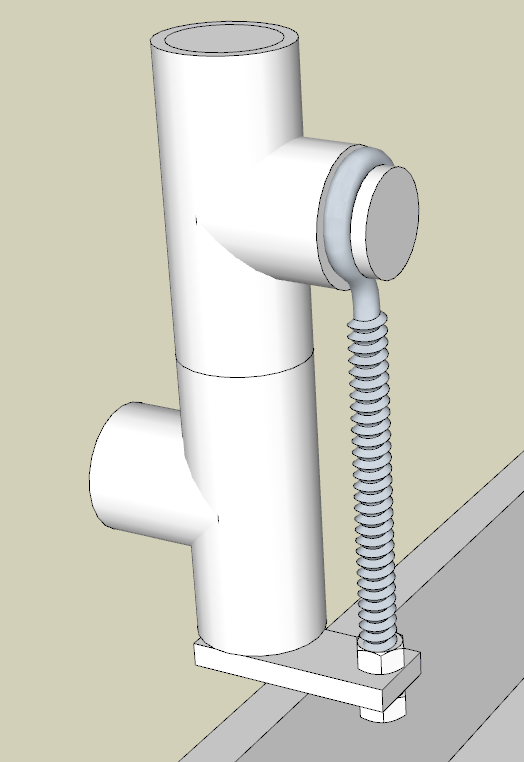
\includegraphics[width=6in, height=3.85in, keepaspectratio]{figures/supply_tubes.png}
	\caption{Supply Tube}	\label{fig:supply_tubes}
\end{figure}
\begin{figure}[H]   % [h] means here
	\centering 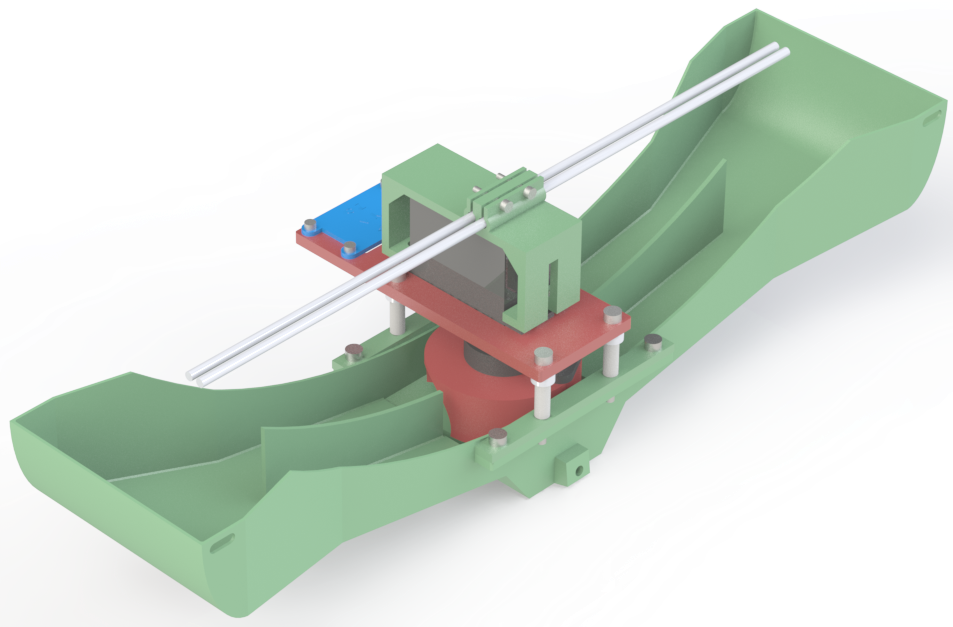
\includegraphics[width=6in, height=3.85in, keepaspectratio]{figures/ball_hopper.png}
	\caption{Ball Hopper}	\label{fig:ball_hopper}
\end{figure}
\begin{figure}[H]   % [h] means here
	\centering 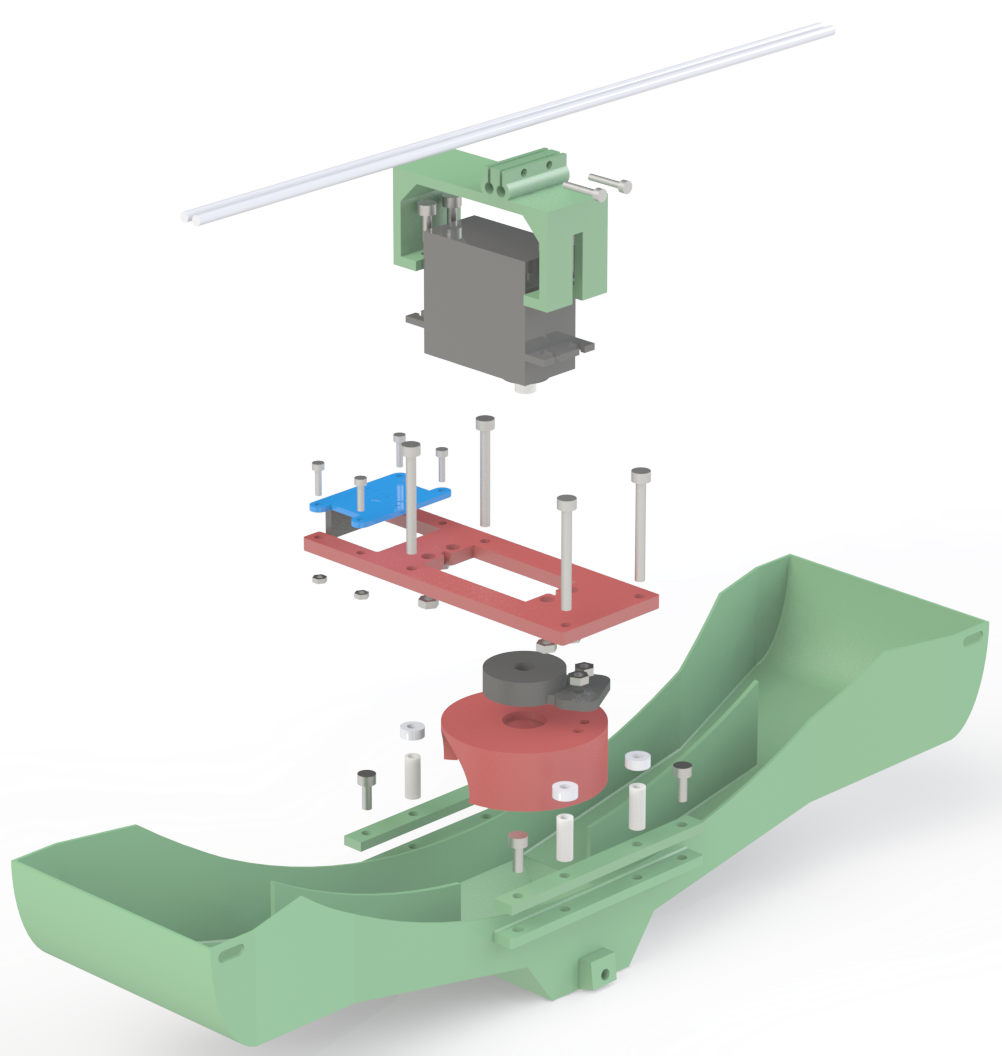
\includegraphics[width=6in, height=3.85in, keepaspectratio]{figures/ball_hopper_explode.png}
	\caption{Ball Hopper -- Exploded View}	\label{fig:ball_hopper_explode}
\end{figure}

To obtain balls, the robot first positions itself such that the wide portion of hopper resides next to the supply tube. The robot then moves such that the metal rods at the top of the ball hopper push the eyebolt aside. As the flap swings open, the balls roll out of the supply tube and down the steep sloped portion of the hopper. Visible in the cross section view of Figure \ref{fig:ball_hopper_xsec}, the slope rapidly becomes shallower in order to convert the balls' downward momentum into sideways momentum which keeps balls from jamming against each other. The balls then roll into one of two channels before stopping at the dispensing gate.

\begin{figure}[H]   % [h] means here
	\centering 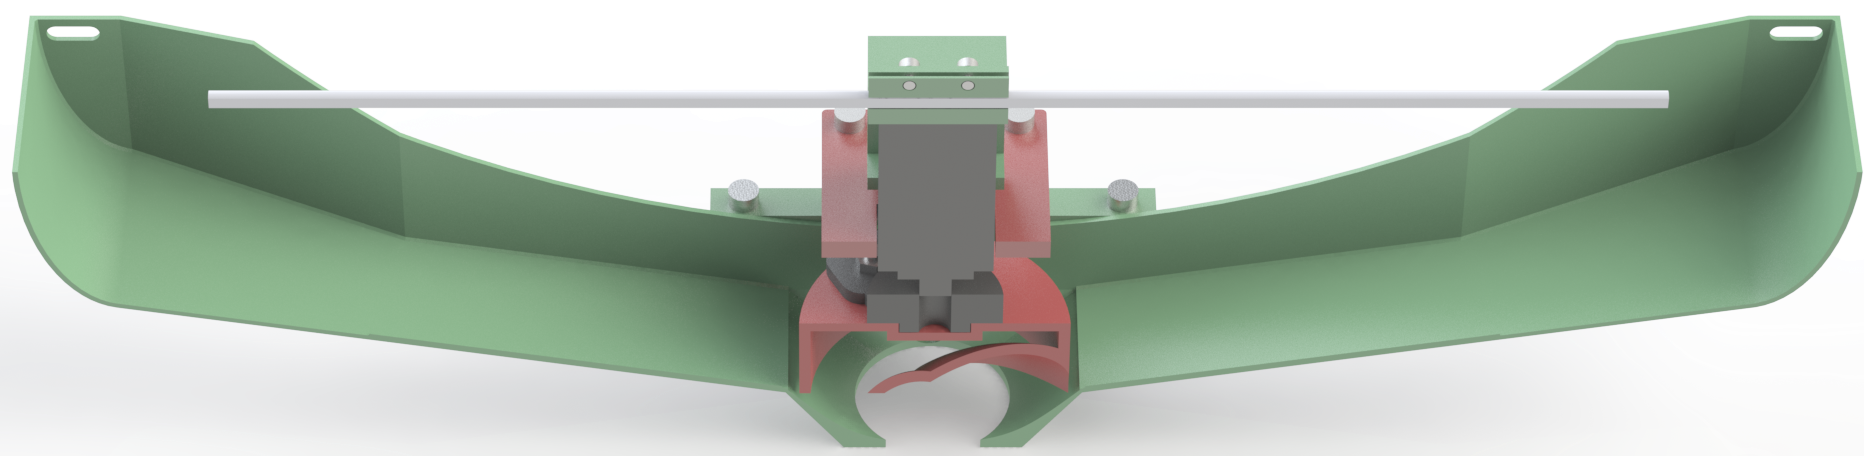
\includegraphics[width=6in, height=3.85in, keepaspectratio]{figures/ball_hopper_xsec.png}
	\caption{Ball Hopper -- Cross Section View}	\label{fig:ball_hopper_xsec}
\end{figure}

The dispensing gate, shown in Figure \ref{fig:dispensing_gate}, controls the movement of balls between hopper channels and the shooting mechanism entrance. Its complex shape directs balls into the hole at the bottom of the ball hopper from one channel at a time to prevent jamming. A standard \ang{180} rotation servo, mounted in a 3D-printed bracket above the center of the hopper, controls the dispensing gate.  Fastened to the same bracket, an inertial measurement unit (IMU) measures magnetic compass heading and acceleration in three dimensions for robot navigation purposes. The IMU is positioned at the rotational center of the robot to prevent the accelerometer from measuring robot rotation as linear movement. The ball hopper is mounted at three points: the top of the shooting mechanism and the left and right edges of the robot using 3D-printed and acrylic braces shown in Figure \ref{fig:hopper_brace}. 
\begin{figure}[H]   % [h] means here
	\centering 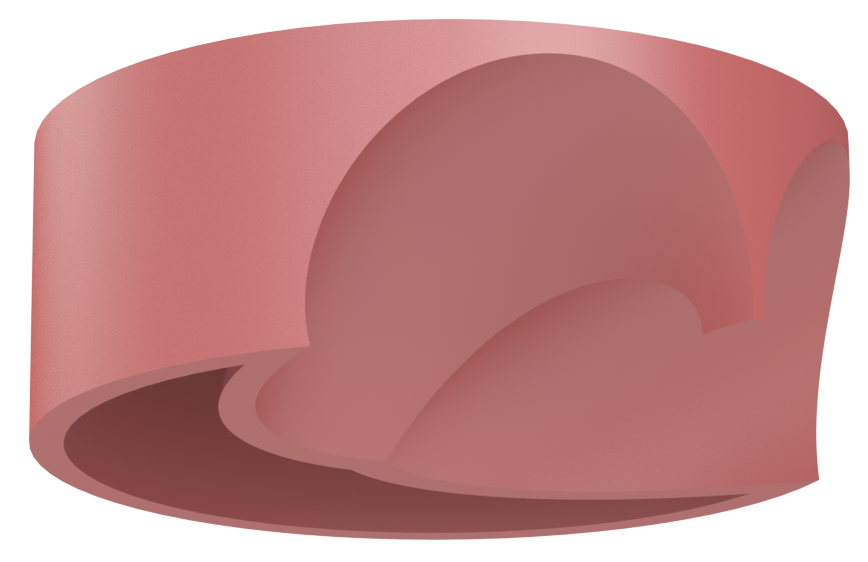
\includegraphics[width=4in, height=3.85in, keepaspectratio]{figures/dispensing_gate.png}
	\caption{Ball Hopper -- Dispensing Gate}	\label{fig:dispensing_gate}
\end{figure}
\begin{figure}[H]   % [h] means here
	\centering 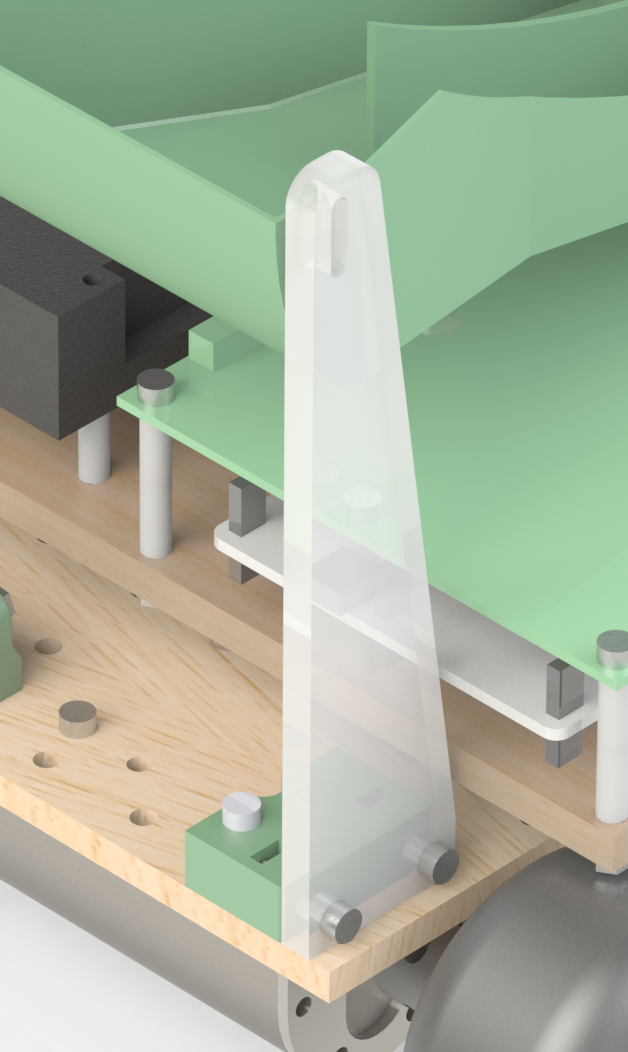
\includegraphics[width=6in, height=5in, keepaspectratio]{figures/hopper_brace.png}
	\caption{Ball Hopper -- Braces}	\label{fig:hopper_brace}
\end{figure}

\section{Control Unit}
The control unit, shown in Figure \ref{fig:control_unit}, consists of a 1/4" MDF board with various electronic components mounted: two off-the-shelf DC-DC switching converters, a custom interconnect printed circuit board (PCB), an off-the-shelf STM32 Nucleo-64 development board, and the Raspberry Pi microcomputer. Two 3D-printed standoffs, shown in Figure \ref{fig:control_unit_standoffs}, connect the control unit to the platform and raise it slightly to avoid colliding with the robot's wheels. 

\begin{figure}[H]   % [h] means here
	\centering 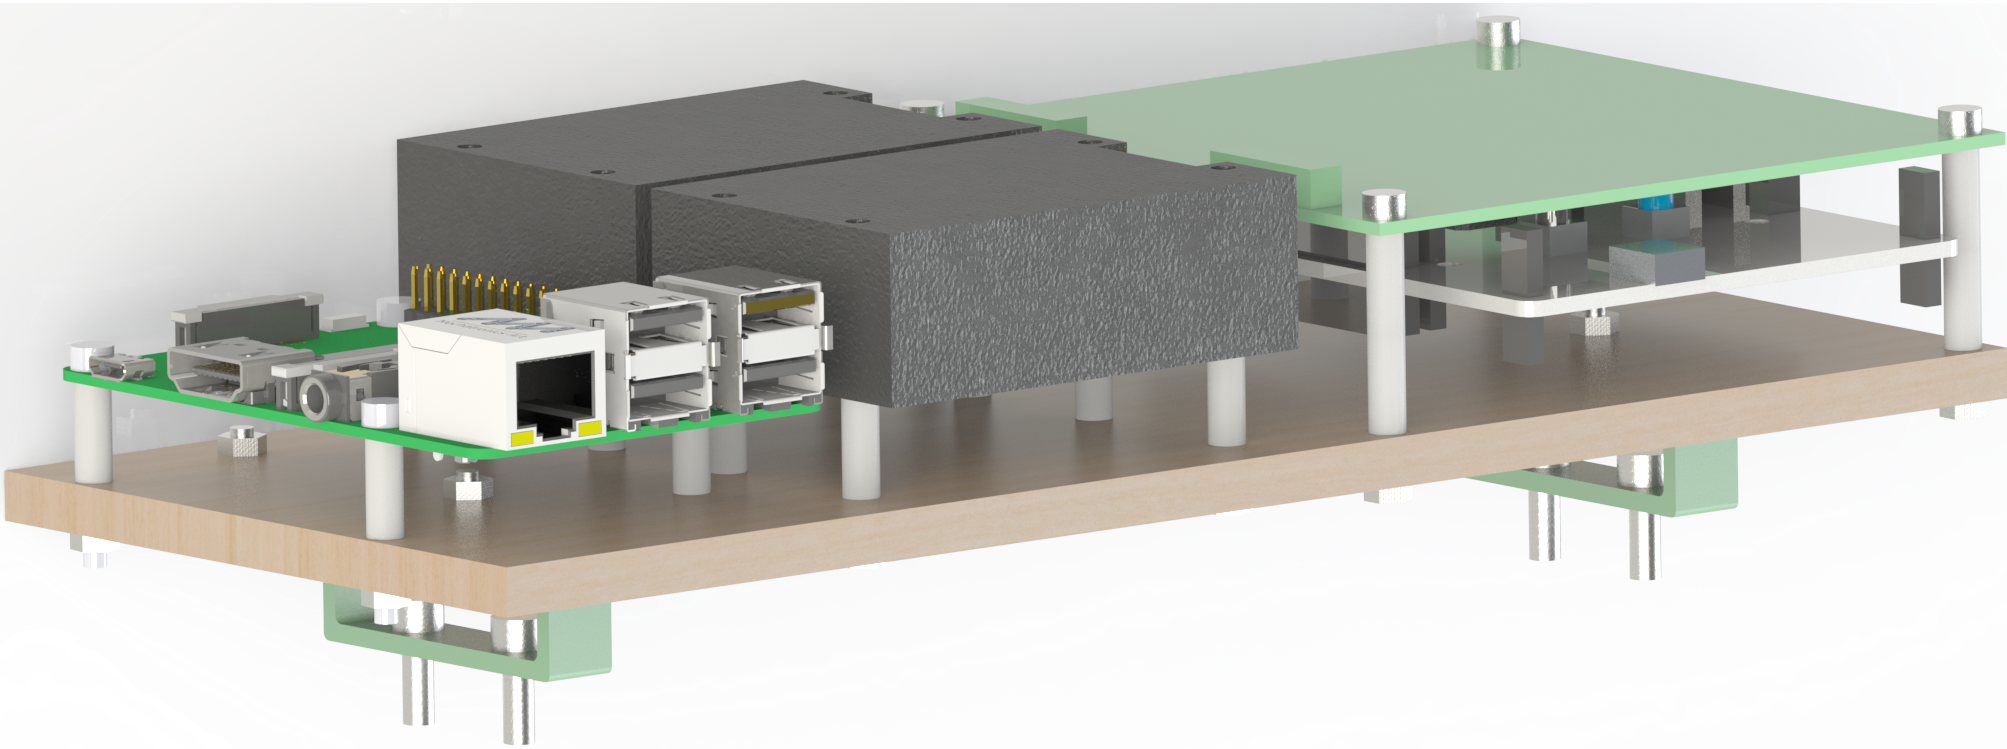
\includegraphics[width=6in, height=3.85in, keepaspectratio]{figures/control_unit.png}
	\caption{Control Unit}	\label{fig:control_unit}
\end{figure}

\begin{figure}[H]   % [h] means here
	\centering 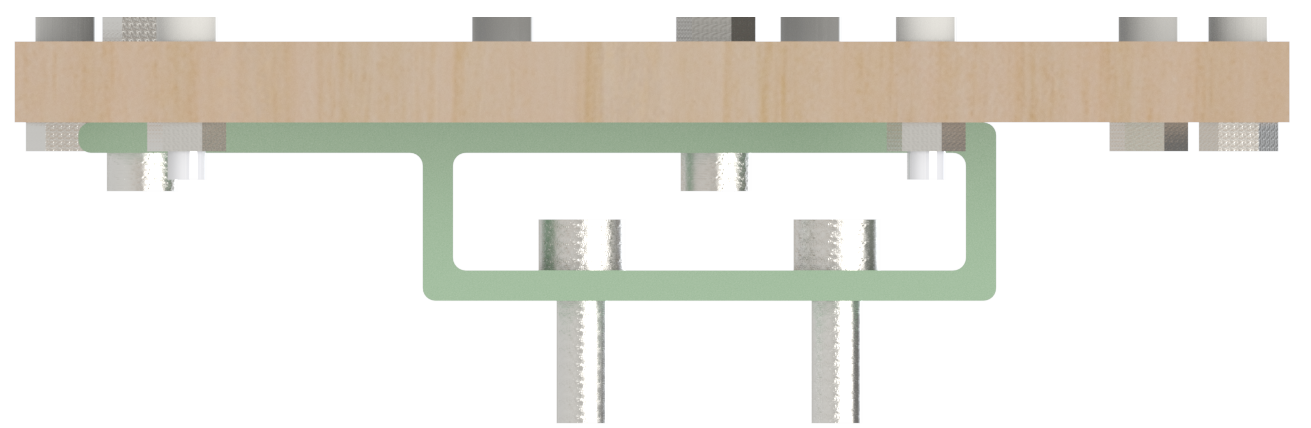
\includegraphics[width=6in, height=3.85in, keepaspectratio]{figures/control_unit_standoffs.png}
	\caption{Control Unit -- Standoffs}	\label{fig:control_unit_standoffs}
\end{figure}

\section{Results and Future Improvements}
The fabrication and assembly of the robot matched the 3D model and parts fit together as expected. Overall, the design can be improved through shrinking components by removing excess material. The close proximity of parts to each other made debugging and troubleshooting difficult.

Due to incomplete modeling of fasteners at the wheels, the base platform interfered slightly with the protruding bolt heads. Ten minutes of sanding the wheel cutouts corrected the issue. Otherwise, the base platform was largely successful. The grid of holes enabled easy relocation of components. Future designs may consider adding wheel suspension to improve traction.

The shooting mechanism underwent three revisions. The first used a belt and pulley system to allow a single slow motor to drive both high-speed launcher wheels, but the large footprint prevented compatibility with other robot components. The second revision was identical to the final iteration except for narrower barrel diameter and a pivot system to allow for aim angle adjustment. After discovering the ball jamming issue, the final iteration used a widened barrel diameter and a fixed aim angle. As described above, the final shooting mechanism was 100\% accurate in 100 trials and satisfied the competition speed limit. The design can be improved by modifying the barrel geometry to shrink the mechanism as it is still quite large.

The ball hopper used two revisions. The first revision used unnecessarily thick walls and extended the channel divider all the way to the edges of the hopper. It also used a shallower initial slope and a ball exit hole positioned in the center instead of offset. Balls would jam in the channel and refuse to fall down the center hole. The final design uses wider channels and a steeper slope to counter jamming problems. Future designs should consider using a single large "bucket" with an indexing agitator similar to the Geneva drive \cite{bickford_1972}.


